\documentclass[a4paper,12pt]{article}
\usepackage{bbding,combelow,textcomp,amsfonts,amsthm,amsmath,amssymb,graphicx,color,hyperref,etoolbox}
\usepackage[utf8x]{inputenc}
\usepackage[lined,boxed,commentsnumbered]{algorithm2e}

\usepackage{tikz}
\usepackage{float}
\usetikzlibrary{positioning}
\usetikzlibrary{arrows.meta}
\usetikzlibrary{calc}

\newtoggle{story}


%%%%%%%%%%%%%%%%%%%%%%%%%%%%%%%%%%%%%%%%%%
%% Customisation options --- update as necessary
%%%%%%%%%%%%%%%%%%%%%%%%%%%%%%%%%%%%%%%%%%

%% Course details: title, semester, instructors

\newcommand{\courseTitle}{Combinatorics II (Math 7702)}
\newcommand{\semester}{Spring 2026}
\newcommand{\instructorA}{Shagnik Das}
\newcommand{\instructorB}{Lu Yun-Chi}

%% Sheet number

\newcommand{\sheetNumber}{2}


%% Submission details

\newcommand{\dueDate}{15:30, Apr 21st.}
\newcommand{\lateWarning}{Late submissions will receive no credit.}


%% Display irrelevant footnotes?  \toggletrue for yes, \togglefalse for no

\toggletrue{story}

%%%%%%%%%%%%%%%%%%%%%%%%%%%%%%%%%%%%%%%%%%
%% End of customisation options
%%%%%%%%%%%%%%%%%%%%%%%%%%%%%%%%%%%%%%%%%%

\pdfpagewidth 8.5in
\pdfpageheight 11in
\topmargin -1in
\headheight 0in
\headsep 0in
\textheight 8.5in
\textwidth 6.5in
\oddsidemargin 0in
\evensidemargin 0in
\headheight 77pt
\headsep 0in
\footskip .75in

\makeatletter
\newcommand{\buildtitle}[4]{
\begin{flushleft}
{\large
#1
\hfill{}
#2
\par
#3
}
\end{flushleft}
\vskip 4pt
\begin{center}
{\large\bfseries#4\par}
\end{center}
\bigskip
}
\makeatother

\renewcommand{\thesection}{\normalsize\arabic{section}}

\renewcommand{\deg}{\textrm{deg}}
\newcommand{\eps}{\varepsilon}
\newcommand{\ceil}[1]{\left \lceil #1 \right \rceil}

\newcommand{\hint}{\begin{flushright} [Hint at \url{\hintURL}.] \end{flushright}}

\newcommand{\card}[1]{\left| #1 \right|}
\newcommand{\mb}[1]{\mathbb{#1}}
\newcommand{\mc}[1]{\mathcal{#1}}


\newcommand{\story}[1]{\iftoggle{story}{\footnote{#1}}{}}
\newcommand{\storymark}[1][42]{\iftoggle{story}{\footnotemark[#1]}{}}
\newcommand{\storytext}[2][42]{\iftoggle{story}{\footnotetext[#1]{#2}}{}}

\newcommand{\bonus}[2]{\paragraph{Bonus (#1 pt\ifstrequal{#1}{1}{}{s})} #2}


\begin{document}


\buildtitle{\courseTitle{}}{\semester}{\instructorA{} \hfill \instructorB{}}{Exercise Sheet \sheetNumber{}}

\vspace{-0.2in}

\begin{center}

{B13902024 Chang, Yi-Kuei \\ \bf Due date: \dueDate \\ \lateWarning}

\end{center}

\noindent You should try to solve all of the exercises below, and then submit two solutions to be graded --- each problem is worth $10$ points. Make sure to clearly justify your answers, defining everything precisely and stating any results you are using. You should then submit your solutions on NTU COOL, either as a typed PDF or a clear picture or scan of your handwritten answers.

\medskip

\noindent The next couple of exercises concern SAT --- the Boolean satisfiability problem --- for which we now define the necessarily terminology.  A \emph{Boolean variable} is a variable that can take one of two variables: True or False.  A \emph{Boolean formula} $f(x_1, x_2, \hdots, x_n)$ is simply a function $f: \{\textrm{True}, \textrm{False} \}^n \rightarrow \{ \textrm{True}, \textrm{False} \}$.  In other words, it takes as input a number of Boolean variables, $x_1, x_2, \hdots, x_n$, and for every possible truth assignment to these variables, evaluates to either True or False.  A Boolean formula $f$ is said to be \emph{satisfiable} if there is some assignment of truth values to its inputs for which $f$ evaluates to True.

Every Boolean formula can be represented by combining the Boolean input variables with three logical operators: `$\wedge$' (and), `$\vee$' (or) and `$\neg$' (not).  In particular, every formula has a \emph{Conjunctive Normal Form (CNF)}.  A \emph{literal} is either a variable $x_i$ or its negation $\neg x_i$.  A \emph{clause} is the `or' of several literals, so it is satisfied if any one of its literals is.  Finally, the CNF formula is the `and' of all its clauses, and is thus satisfied if and only if all of its clauses are.  The Boolean satisfiability problem is the decision problem asking whether or not a given CNF formula is satisfiable.

A $k$-CNF formula consists of clauses with exactly $k$ literals\footnote{Some authors would only ask that there only be at most $k$ literals.  However, these are essentially equivalent, since given a clause $C$ with fewer than $k$ literals, we can introduce a new variable $y$, and replace $C$ with the logically-equivalent $(C \vee y) \wedge (C \vee \neg y)$.}, each corresponding to different variables\footnote{Having literals with the same variable is redundant: $x \vee x$ is just $x$, while $x \vee \neg x$ is always True.}.  For example, the following is a $4$-CNF formula:
\[ f(x_1, x_2, x_3, x_4, x_5, x_6) = \left( x_1 \vee \neg x_2 \vee x_4 \vee \neg x_5 \right) \wedge \left(x_2 \vee x_3 \vee \neg x_4 \vee x_6 \right) \wedge \left( x_1 \vee \neg x_2 \vee x_5 \vee \neg x_6 \right).\]
This formula is satisfiable, since, for example, $f(\textrm{True},\textrm{False}, \textrm{True}, \textrm{True}, \textrm{False}, \textrm{False}) = \textrm{True}$.  In general, the $k$-satisfiability ($k$-SAT) problem is the Boolean satisfiability problem restricted to $k$-CNFs.

\paragraph{Exercise 1}
\begin{itemize}
	\item[(a)] Provide an example of an unsatisfiable instance of $k$-SAT.
	\item[(b)] Show that every instance of $k$-SAT with fewer than $2^k$ clauses must be satisfiable.
\end{itemize}

\paragraph{Exercise 2}  
\begin{itemize}
	\item[(a)] Show that $2$-SAT is in $\mc P$.
	\item[(b)] Prove that for every $k \ge 4$, $k$-SAT can be (polynomially) reduced to $3$-SAT. That is, given a $k$-CNF formula $f_k$, you can in polynomial time build a $3$-CNF formula $f_3$ that is satisfiable if and only if $f_k$ is. 
\end{itemize}

\paragraph{Exercise 3}  In this exercise, you will extend Tutte's theorem to give certificates for maximum matchings and not just perfect matchings.

Prove that for every graph $G = (V, E)$, we have
\[ 2 \alpha'(G) = \min_{S \subseteq V} \left( \card{V} + \card{S} - o( G \setminus S ) \right). \]

\paragraph{Solution:} Set $n:=|V|$, and define the \emph{deficiency}
\[
\operatorname{def}(G):=\max_{S\subseteq V}\bigl(o(G-S)-|S|\bigr).
\]
The claimed identity is equivalent to
\[
\alpha'(G)=\frac{n-\operatorname{def}(G)}{2}.
\]

First, we show $n-2\alpha'(G)\ge \operatorname{def}(G)$. Let $M$ be any matching.
Fix $S\subseteq V$. Consider odd components of $G-S$.
In an odd component $C$, edges of $M$ internal to $C$ cover an even number of vertices;
therefore at least one vertex of $C$ is either unmatched by $M$ or matched by an edge going from $C$ to $S$.
Each vertex of $S$ is incident to at most one matching edge, so at most $|S|$ odd components can be ``accounted for'' by such edges to $S$.
Hence at least $o(G-S)-|S|$ odd components contain a vertex unmatched by $M$.
So the total number of unmatched vertices, namely $n-2|M|$, satisfies
\[
n-2|M|\ge o(G-S)-|S|.
\]
Since this holds for every $S$, we get
\[
n-2|M|\ge \operatorname{def}(G).
\]
Taking $|M|=\alpha'(G)$ gives
\[
n-2\alpha'(G)\ge \operatorname{def}(G).\tag{1}
\]

For the reverse inequality, let $d:=\operatorname{def}(G)$.
By parity, $d\equiv n \pmod 2$ (because $o(G-S)\equiv |V\setminus S|$ mod $2$ for every $S$).
Hence $n+d$ is even.

Now form the graph
\[
H:=G\vee K_d
\]
(join $G$ with a complete graph on $d$ new vertices).
We claim $H$ has a perfect matching.
By Tutte's 1-factor theorem, it is enough to show
\[
o(H-T)\le |T| \quad \text{for all } T\subseteq V(H).
\]
Write $T=S\cup R$, where $S\subseteq V(G)$ and $R\subseteq V(K_d)$.

If $R\neq V(K_d)$, then at least one vertex of $K_d$ remains in $H-T$; because that vertex is adjacent to every remaining vertex of $G$, all vertices of $H-T$ lie in one connected component. Thus $o(H-T)\le 1\le |T|$ unless $T=\varnothing$; and for $T=\varnothing$, $|V(H)|=n+d$ is even, so $o(H)=0$.

If $R=V(K_d)$, then $H-T=G-S$, so
\[
o(H-T)=o(G-S)\le |S|+d=|T|,
\]
because $d=\max_{X\subseteq V}(o(G-X)-|X|)$.

Therefore Tutte's condition holds, and $H$ has a perfect matching $P$.
Restrict $P$ to edges of $G$: this gives a matching $M$ in $G$.
At most $d$ vertices of $G$ can be matched in $P$ to vertices of $K_d$, so at least $n-d$ vertices of $G$ are matched within $G$.
Hence
\[
|M|\ge \frac{n-d}{2},
\]
so
\[
\alpha'(G)\ge \frac{n-d}{2}
\quad\Longrightarrow\quad
n-2\alpha'(G)\le d=\operatorname{def}(G).\tag{2}
\]

Combining (1) and (2):
\[
n-2\alpha'(G)=\operatorname{def}(G).
\]
Rewriting,
\[
2\alpha'(G)=n-\max_{S\subseteq V}\bigl(o(G-S)-|S|\bigr)
=\min_{S\subseteq V}\bigl(n+|S|-o(G-S)\bigr),
\]
which is exactly the formula.

\begin{figure}[H]
\centering
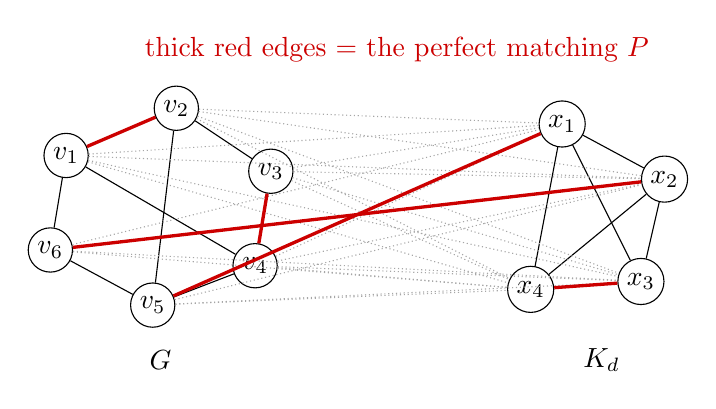
\begin{tikzpicture}[
    scale=1,
    vtx/.style={circle, draw, inner sep=1.8pt},
    edgeG/.style={black},
    edgeJoin/.style={densely dotted, gray!70},
    edgeM/.style={very thick, red!80!black}
]
    % vertices of G
    \node[vtx] (g1) at (0,2.2) {$v_1$};
    \node[vtx] (g2) at (1.4,2.8) {$v_2$};
    \node[vtx] (g3) at (2.6,2.0) {$v_3$};
    \node[vtx] (g4) at (2.4,0.8) {$v_4$};
    \node[vtx] (g5) at (1.1,0.3) {$v_5$};
    \node[vtx] (g6) at (-0.2,1.0) {$v_6$};

    % some edges inside G
    \draw[edgeG] (g1)--(g2)--(g3)--(g4)--(g5)--(g6)--(g1);
    \draw[edgeG] (g2)--(g5);
    \draw[edgeG] (g1)--(g4);

    % vertices of K_d
    \node[vtx] (k1) at (6.3,2.6) {$x_1$};
    \node[vtx] (k2) at (7.6,1.9) {$x_2$};
    \node[vtx] (k3) at (7.3,0.6) {$x_3$};
    \node[vtx] (k4) at (5.9,0.5) {$x_4$};

    % complete graph on K_d vertices
    \draw[edgeG] (k1)--(k2)--(k3)--(k4)--(k1);
    \draw[edgeG] (k1)--(k3);
    \draw[edgeG] (k2)--(k4);

    % all join edges between V(G) and V(K_d)
    \foreach \gi in {1,2,3,4,5,6} {
        \foreach \kj in {1,2,3,4} {
            \draw[edgeJoin] (g\gi)--(k\kj);
        }
    }

    % sample matching M in H
    \draw[edgeM] (g1)--(g2);
    \draw[edgeM] (g3)--(g4);
    \draw[edgeM] (g5)--(k1);
    \draw[edgeM] (g6)--(k2);
    \draw[edgeM] (k3)--(k4);

    \node[draw=none] at (1.2,-0.4) {$G$};
    \node[draw=none] at (6.8,-0.4) {$K_d$};
    \node[draw=none, text=red!80!black] at (4.2,3.55) {thick red edges $=$ the perfect matching $P$};
\end{tikzpicture}
\caption{$H=G\vee K_d$.}
\label{fig:join}
\end{figure}

\paragraph{Exercise 4}  A graph $G = (V,E)$ is called \emph{cubic} if every vertex has degree three, and \emph{bridgeless} if we have to remove at least two edges to disconnect $G$.
\begin{itemize}
	\item[(a)] Give an example of a cubic graph that does not have a perfect matching.
	\item[(b)] Prove that every cubic bridgeless graph has a perfect matching.
\end{itemize}

\paragraph{Solution:}
\begin{itemize}
	\item [(a)] We give the example of the below graph:
	\begin{figure}[H]
		\centering
		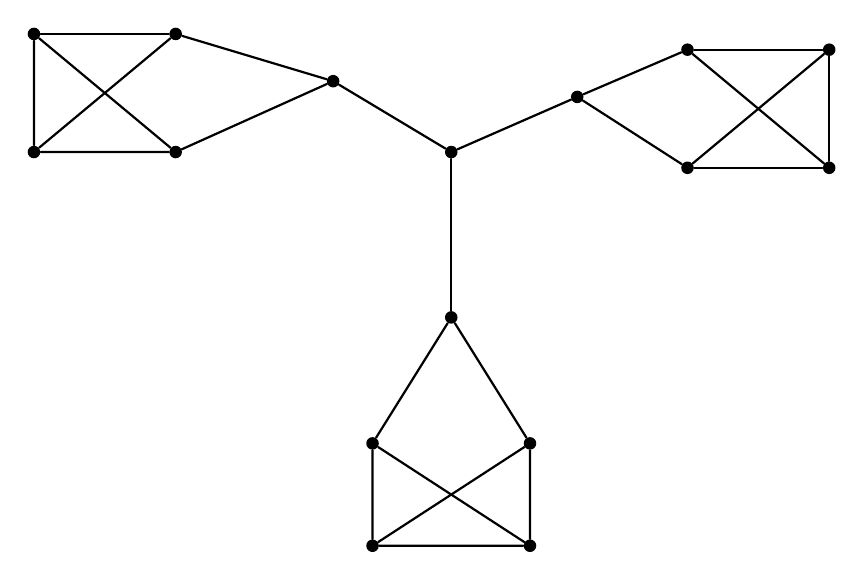
\begin{tikzpicture}[
			x=1cm,
			y=1cm,
			line cap=round,
			line join=round,
			every node/.style={circle, fill, inner sep=1.6pt}
		]
		% Left block
		\node (L1) at (0.0, 3.5) {};
		\node (L2) at (0.0, 2.0) {};
		\node (L3) at (1.8, 3.5) {};
		\node (L4) at (1.8, 2.0) {};

		% Top chain and junctions
		\node (M1) at (3.8, 2.9) {};
		\node (C)  at (5.3, 2.0) {};
		\node (R1) at (6.9, 2.7) {};
		\node (R2) at (8.3, 3.3) {};

		% Right block
		\node (R3) at (10.1, 3.3) {};
		\node (R4) at (8.3, 1.8) {};
		\node (R5) at (10.1, 1.8) {};

		% Bottom house
		\node (B0) at (5.3, -0.1) {};
		\node (B1) at (4.3, -1.7) {};
		\node (B2) at (6.3, -1.7) {};
		\node (B3) at (4.3, -3.0) {};
		\node (B4) at (6.3, -3.0) {};

		% Left block edges
		\draw[thick] (L1) -- (L2) -- (L4) -- (L1);
		\draw[thick] (L1) -- (L3);
		\draw[thick] (L2) -- (L3);

		% Middle top edges
		\draw[thick] (L3) -- (M1);
		\draw[thick] (L4) -- (M1);
		\draw[thick] (M1) -- (C);
		\draw[thick] (C) -- (B0);
		\draw[thick] (C) -- (R1);
		\draw[thick] (R1) -- (R2);

		% Right block edges
		\draw[thick] (R2) -- (R3);
		\draw[thick] (R4) -- (R5) -- (R3) -- cycle;
		\draw[thick] (R2) -- (R5);
		\draw[thick] (R4) -- (R3);
		\draw[thick] (R1) -- (R4);

		% Bottom house edges
		\draw[thick] (B0) -- (B1) -- (B3) -- (B4) -- (B2) -- cycle;
		\draw[thick] (B0) -- (B2);
		\draw[thick] (B1) -- (B4);
		\draw[thick] (B2) -- (B3);
		\end{tikzpicture}
	\end{figure}
	This graph is cubic, but if we remove the middle vertex of this graph, the remaining graph has three odd components, so by Tutte's theorem, this graph does not have a perfect matching.
	\item [(b)] It suffices to show that every cubic bridgeless graph \(G=(V,E)\) has \(\forall S \subseteq V(G)\), \(o(G - S) \le \vert S \vert \) by Tutte's theorem. Now given some \(S \subseteq V(G)\). If \(C_1, \dots , C_k\) are all odd componenets of \(G - S\), then suppose \(p_i = \# \) of edges between \(S\) and all odd \(C_i\) for all \(1 \le i \le k\), we have 
	\[
		p_i = 3 \vert C_i \vert - 2 \vert E(C) \vert \quad \forall 1 \le i \le k,  
	\]
	since every vertex in \(C_i\) has degree 3, and \(p_i\) is the sum of the number of edges incident to every vertex in \(C_i\) minus the number of edges between two vertices of \(C_i\). Thus, we know \(p_i\) is odd for all \(1 \le i \le k\) since \(\vert C_i \vert \) is odd and \(2 \vert E(C) \vert \) is even. Also, since \(G\)  is bridgesless, there is at least 3 edges between \(C_i\) and \(S\) for all \(1 \le i \le k\), so we can count the number of edges between \(S\) and all \(C_i\)s. Hence,
	\[
		3 o(G - S) \le \# \text{ of edges between } C_i \text{'s} \le 3 \vert S \vert      
	\]            
	since at most all edges in \(S\) are incident to \(C_i\) for some \(1 \le i \le k\). Thus, we have \(3 o(G - S) \le 3 \vert S \vert \), and we're done.     
\end{itemize}

\paragraph{Exercise 5} Use the Hungarian Algorithm, showing all the key steps, to find a \emph{minimum}-weight matching in $K_{5,5}$ with the edge weights $W = \left( \omega_{i,j} \right)$ as below, and then give a short proof that your matching is optimal.

\[ W = \begin{pmatrix}
	4 & 5 & 8 & 10 & 11 \\
	7 & 6 & 5 & 7 & 4 \\
	8 & 5 & 12 & 9 & 6 \\
	6 & 6 & 13 & 10 & 7 \\
	4 & 5 & 7 & 9 & 8
\end{pmatrix} . \]

%\newpage

%\section*{Hints}  The following QR codes contain hints for some of the homework exercises.  You should be able to decode them using any QR code scanner, including this one: \url{https://zxing.org/w/decode.jspx}.

%\paragraph{Exercise 4} Also available at \url{https://i.ibb.co/1GnLG3LJ/S2E4.png}.

%\begin{center}
%	\includegraphics[scale=0.5]{Hints/S2E4.png}
%\end{center}

\end{document}